\documentclass[11pt]{article}
\usepackage[preprint]{acl}
\usepackage{times}
\usepackage{latexsym}
\usepackage[T1]{fontenc}
\usepackage[utf8]{inputenc}
\usepackage{inconsolata}

\usepackage{amsmath}
\usepackage{amssymb}
\usepackage{booktabs}
\usepackage{graphicx}
\usepackage{microtype}
\usepackage{url}
\usepackage{hyperref}

% ACL defines 10 pt captions. Explicitly keep every figure caption roman.
\captionsetup[figure]{font={10pt,rm},labelfont=rm,textfont=rm}
\graphicspath{{figures/}}

\newcommand{\Rsem}{R_{\mathrm{sem}}}
\newcommand{\Rrnd}{R_{\mathrm{rnd}}}
% BEGIN GENERATED RTX RESULTS
% Generated from measured results.
\newcommand{\ExpOneTransitionLow}{0.06}
\newcommand{\ExpOneTransitionHigh}{0.98}
\newcommand{\ExpTwoAttribute}{1.000}
\newcommand{\ExpOneSemanticProbe}{0.990}
\newcommand{\ExpOneSemanticProbeStats}{0.990\pm0.007}
\newcommand{\ExpOneSemanticTrained}{0.672}
\newcommand{\ExpOneSemanticTrainedStats}{0.672\pm0.122}
\newcommand{\ExpOneSemanticHeldout}{0.635}
\newcommand{\ExpOneSemanticHeldoutStats}{0.635\pm0.182}
\newcommand{\ExpOneRandomProbe}{0.036}
\newcommand{\ExpOneRandomProbeStats}{0.036\pm0.007}
\newcommand{\ExpOneRandomTrained}{0.167}
\newcommand{\ExpOneRandomTrainedStats}{0.167\pm0.035}
\newcommand{\ExpOneRandomHeldout}{0.031}
\newcommand{\ExpOneRandomHeldoutStats}{0.031\pm0.000}
\newcommand{\ExpOneAffine}{0.965\pm0.010}
\newcommand{\ExpOneMidpoint}{0.352\pm0.011}
\newcommand{\ExpOneJacobian}{0.281\pm0.013}
\newcommand{\ExpOneTangent}{0.284\pm0.013}
\newcommand{\ExpOneValuePatch}{0.987\pm0.008}
\newcommand{\ExpOnePatternPatch}{0.013\pm0.007}
\newcommand{\ExpOneHeadsPresent}{0.729\pm0.094}
\newcommand{\ExpOneRelationPatch}{0.850\pm0.017}
\newcommand{\ExpOneTopOnly}{0.498\pm0.029}
\newcommand{\ExpOneTopAblated}{0.790\pm0.032}
\newcommand{\ExpTwoMinStructured}{0.9998}
\newcommand{\ExpTwoMinStructuredStats}{0.99976\pm0.00000}
\newcommand{\ExpTwoRandom}{0.9998}
\newcommand{\ExpTwoRandomStats}{0.99984\pm0.00014}
\newcommand{\ExpTwoSymmetry}{0.9995}
\newcommand{\ExpTwoSymmetryStats}{0.99951\pm0.00000}
\newcommand{\ExpTwoStructuredRsq}{0.995}
\newcommand{\ExpTwoStructuredRsqStats}{0.99527\pm0.00042}
\newcommand{\ExpTwoRandomRsq}{0.375}
\newcommand{\ExpTwoRandomRsqStats}{0.37493\pm0.03116}
\newcommand{\ExpTwoStructuredMeanRsq}{0.99697}
\newcommand{\ExpTwoStructuredLowestRsq}{0.99485}
\newcommand{\ExpTwoRandomRsqSeeds}{0.384, 0.401, and 0.340}
\newcommand{\ExpTwoRandomErrors}{0.785, 0.774, and 0.812}
\newcommand{\ExpTwoNullPercentiles}{94.8, 98.0, and 49.2}
\newcommand{\ExpTwoNullMean}{0.339}
\newcommand{\ExpTwoRandomFull}{1.000\pm0.000}
\newcommand{\ExpTwoRandomFullPrecise}{0.99984\pm0.00014}
\newcommand{\ExpTwoStructuredFull}{1.000\pm0.000}
\newcommand{\ExpTwoStructuredFullPrecise}{0.99995\pm0.00000}
\newcommand{\ExpTwoRandomGelu}{0.510\pm0.008}
\newcommand{\ExpTwoRandomGeluPrecise}{0.51017\pm0.00754}
\newcommand{\ExpTwoStructuredGelu}{0.551\pm0.043}
\newcommand{\ExpTwoStructuredGeluPrecise}{0.55110\pm0.04267}
\newcommand{\ExpTwoRandomUniform}{0.498\pm0.003}
\newcommand{\ExpTwoRandomUniformPrecise}{0.49821\pm0.00289}
\newcommand{\ExpTwoStructuredUniform}{0.498\pm0.007}
\newcommand{\ExpTwoStructuredUniformPrecise}{0.49825\pm0.00656}
\newcommand{\ExpTwoRandomNoMlp}{0.531\pm0.014}
\newcommand{\ExpTwoRandomNoMlpPrecise}{0.53068\pm0.01403}
\newcommand{\ExpTwoStructuredNoMlp}{0.599\pm0.022}
\newcommand{\ExpTwoStructuredNoMlpPrecise}{0.59911\pm0.02229}
\newcommand{\ExpTwoRandomNoAttention}{0.500\pm0.000}
\newcommand{\ExpTwoRandomNoAttentionPrecise}{0.50000\pm0.00000}
\newcommand{\ExpTwoStructuredNoAttention}{0.500\pm0.000}
\newcommand{\ExpTwoStructuredNoAttentionPrecise}{0.50000\pm0.00000}
\newcommand{\ExpTwoLens}{0.500, 0.503, 0.505, 0.522, 0.535, 0.518, 0.620, 0.665, and 0.9998}
\newcommand{\ExpTwoAttentionRange}{0.597--0.714}
\newcommand{\ExpTwoMlpRange}{0.691--0.916}
\newcommand{\ExpTwoSubjectTrace}{1.000, 0.684, 0.650, 0.442, 0.414, 0.363, 0.254, 0.107, and 0.000}
\newcommand{\ExpTwoObjectTrace}{0.000, 0.235, 0.426, 0.548, 0.577, 0.639, 0.764, 0.922, and 1.000}
% END GENERATED RTX RESULTS

\title{Semantic Structure Defines Relation Geometry in Transformers}
% \title{Semantic Structure and Relation Geometry in
%   Transformers: Synthetic vs Natural Language Data}



% Grouped names and numbered affiliations in the native ACL title block.
\author{%
\textbf{Jonas Rohweder\textsuperscript{1,2,3}\hspace{0.9in}%
Hinrich Sch{\"u}tze\textsuperscript{1,3}}\\[0.6em]
\normalfont
\textsuperscript{1}Center for Information and Language Processing (CIS), LMU Munich\\
\textsuperscript{2}Ubiquitous Knowledge Processing Lab (UKP Lab), TU Darmstadt\\
\textsuperscript{3}Munich Center for Machine Learning (MCML)%
}
\hypersetup{hidelinks,
  pdftitle={Semantic Structure Defines Relation Geometry in Transformers},
  pdfauthor={Jonas Rohweder, Hinrich Schütze},pdfsubject={},pdfkeywords={}}

\newcounter{notecounter}
\newcommand{\enotesoff}{\long\gdef\enote##1##2{}}
\newcommand{\enoteson}{\long\gdef\enote##1##2{{
\stepcounter{notecounter}
{\large\bf
\hspace{0cm}\arabic{notecounter} $<<<$ ##1: ##2
$>>>$\hspace{1cm}}}}}

\enoteson
\enotesoff


\begin{document}

\maketitle


\begin{abstract}

%\enote{hs}{
%   We separate three properties that are
%often conflated: recalling a relation, representing it with an affine map, and
%executing it with affine computation. --
%Component interventions show that the forward computation requires
%content-dependent attention and GELU MLPs. --
%As far as the
%abstract is concerned: maybe we shouldn't
%cover this  since it would be quite difficult
%to do this part justice in the available space?}


Prior work links the emergence of linear relational representations in language
models to how often a relation appears in pretraining data. We show that corpus
frequency alone does not determine relational linearity; instead, \emph{semantic
structure}---the attributes that subjects and objects share---plays a central
role. We construct two controlled synthetic settings, A and B. In A, a
transformer sees each training fact of an attribute-defined relation $\Rsem$ at
low frequency, yet a linear probe transfers to held-out subjects with
\ExpOneSemanticProbe{} accuracy and the model recalls held-out objects at
\ExpOneSemanticHeldout{}. A frequency-matched random relation $\Rrnd$ without
attribute structure remains at chance ($1/32$). In B, a transformer sees a
random relation $\Rrnd$ ten times as often in joint training as each of ten
attribute-defined relations $r_i$ (50\% vs.\ 5\% of relation examples).
Although the model memorizes $\Rrnd$ at \ExpTwoRandom{} accuracy, fitting a
linear map from subject to target object embeddings yields only
$R^2=\ExpTwoRandomRsq{}$, compared with \ExpTwoStructuredRsq{} for the $r_i$.
Consistently, in the pretrained LMEnt-1B model, linear relational
embedding (LRE) faithfulness tracks many-to-one object sharing rather than pair
co-occurrence frequency.
Code is available at \url{https://github.com/jonasrohw/affine-structure-defines-linear-geometry}.

\end{abstract}

\begin{figure*}[t]
  \centering
  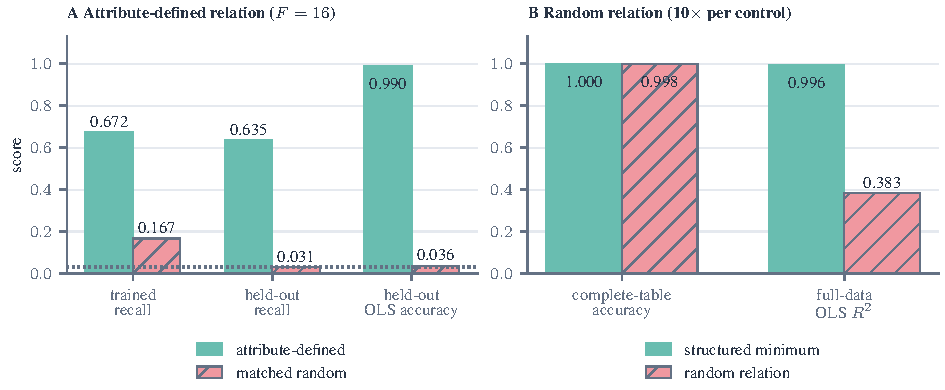
\includegraphics[width=1.0\textwidth]{frequency_not_enough.pdf}
  \caption{Exposure frequency does not determine linear relation geometry in the
  two controlled settings (bars show means over three seeds). \textbf{A (Low
  exposure):} At 16 occurrences per trained triple, the attribute-defined
  relation (solid) generalizes to held-out subjects in both model recall and
  ordinary least squares (OLS) linear probe transfer, whereas the
  frequency-matched random control (hatched) remains at chance ($1/32$).
  \textbf{B (High exposure):} During joint training, the random relation
  receives 50\% of each batch---ten times the 5\% share of each of the ten
  structured attribute-equality controls. The model memorizes both nearly
  perfectly, but the random relation's full-data linear regression $R^2$ remains
  far below the minimum across the ten structured relations.}
  \label{fig:summary}
\end{figure*}


\section{Introduction}
Pretrained transformer language models \citep{vaswani2017attention,brown2020language}
often encode factual relations as \emph{linear relational embeddings} (LREs),
where a single relation-specific linear transformation maps subject
representations to object representations
\citep{hernandez2024linearity,valer2026relational}. \citet{merullo2025frequency}
find that LRE faithfulness correlates strongly with subject--object
co-occurrence frequency in pretraining data, suggesting that linear relational
representations emerge once a relation crosses a co-occurrence threshold.
Exposure frequency is therefore a natural candidate for explaining when
relational linearity arises. However, corpus frequency in natural text is confounded with semantic
structure: frequently stated relations often connect entities that share
underlying attributes reinforced across the rest of the corpus.

Our analysis of the pretrained LMEnt-1B model motivates separating these
factors: within individual relations, facts with more pretraining
co-occurrences are no more likely to be decoded by a relation's LRE once answer
sharing is taken into account (Section~\ref{sec:lment-frequency}). To test
whether exposure frequency or semantic structure drives relational linearity, we
construct two synthetic pretraining settings that vary exposure and attribute
structure independently. Interpreting these experiments requires distinguishing
three properties that can dissociate: \emph{behavior} (whether the model
outputs the correct object), \emph{representation geometry} (whether a linear
transformation between entity embeddings predicts the target), and
\emph{executed computation} (whether the transformer's forward pass is itself
linear in the input). Figure~\ref{fig:summary} previews how these properties
separate across our two settings.

A rarely stated relation can draw on structure learned from other facts. If a
corpus establishes that several towns are in France, stating the official
language for only a few of them can support the same mapping for the rest, even
when a specific town--language pair rarely or never co-occurs. Experiment~A
tests this mechanism by defining a relation $\Rsem$ through entity attributes
learned separately in the corpus, paired with a frequency-matched random
relation $\Rrnd$ over the same entities. Attribute training organizes the token
embeddings into a linearly decodable geometry even before the model reliably
recalls the relation triples. Once recall emerges, both the model and a linear
probe generalize to held-out subjects, whereas the frequency-matched random
relation remains at chance.

Conversely, high exposure alone should not induce linear geometry when paired
entities share no underlying attributes. Repeating an arbitrary set of
subject--object pairs allows a model to memorize every pairing, but without
attribute overlap across the related entities, no shared direction forms in
embedding space to align subjects linearly with their targets. Experiment~B
tests this regime by training a decoder-only transformer on a random relation
$\Rrnd$ alongside ten attribute-defined relations $r_i$, where $\Rrnd$ appears
ten times as often in joint training as each $r_i$ (50\% vs.\ 5\% of relation
examples). Although the transformer learns the $r_i$ and memorizes $\Rrnd$ at
99.98\% accuracy, fitting a linear map from subject to target object embeddings
yields only $R^2=\ExpTwoRandomRsq{}$ on $\Rrnd$, compared with
\ExpTwoStructuredRsq{} on the $r_i$.

Together, our experiments support three conclusions:

\begin{itemize}
  \item Low direct exposure suffices for linear representation geometry when
  other training facts organize entities along the relevant attributes.
  \item High exposure of an arbitrary relation does not induce a linear
  representation of that relation, even when a decoder-only transformer with
  trainable embeddings memorizes the relation nearly perfectly.
  \item Linear decodability of embeddings does not imply linear forward
  computation: Experiment~A exhibits strong linear embedding transfer alongside
  a nonlinear forward pass, while Experiment~B relies on distributed nonlinear
  attention and MLP layers to execute its memorized lookup.
\end{itemize}



\section{Three levels of relational linearity}
\label{sec:definitions}

We evaluate relational linearity at three distinct levels.
Let $s$ denote a subject, $r$ a relation, and $o$ an object.

\paragraph{Behavior.}
Does the model output the correct object for a given $(s, r)$ query? We measure
recall or classification accuracy on the target relation table. High behavioral
accuracy establishes that the model has learned the relation, but does not
specify how the relation is represented or computed.

\paragraph{Representation geometry.}
Let $e(s)\in\mathbb{R}^d$ be a subject representation and $t_r(s)$ be the target
representation for relation $r$. Following \citet{hernandez2024linearity} and
\citet{merullo2025frequency}, a relation has a linear relational representation
between $e$ and $t_r$ if a single matrix $M_r$ and bias $b_r$ approximate the
target across subjects:
\begin{equation}
  t_r(s) \approx M_r e(s)+b_r.
  \label{eq:affine-map}
\end{equation}
Whether Equation~\ref{eq:affine-map} holds depends on which representations $e$
and $t_r$ are tested. In our synthetic experiments, we test token embeddings
directly (Section~\ref{sec:design}): Experiment~A fits a linear probe from input
subject token embeddings to output object token embeddings and evaluates
generalization to subjects excluded from relation training, whereas Experiment~B
fits a linear regression from subject token embeddings to the centroid of
positive object embeddings across all 64 memorized entities.

\paragraph{Executed computation.}
Even when token embeddings are related by Equation~\ref{eq:affine-map}, the
transformer's relation-conditioned forward pass $h(x)$ is linear (with an
offset) on the tested domain only if it maps midpoints of inputs to midpoints of
outputs and has a constant input--output Jacobian matrix. Experiment~A tests
departures from these two conditions using midpoint defect and Jacobian
dispersion (Appendix~\ref{app:metrics}), while Experiment~B uses causal
ablations of GELU activations and attention routing to test whether nonlinear
components are necessary for recall. A high linear probe score on embeddings
does not imply a linear forward pass, and a nonlinear forward pass does not
preclude linear embedding geometry.

\section{Related work}

\paragraph{Linear relational representations.}
\citet{hernandez2024linearity} show that linear relational embeddings (LREs)
decode a wide range of factual relations from intermediate hidden states in
transformer language models. \citet{marconato2025all} analyze when linear
properties of next-token predictors are identifiable, and
\citet{valer2026relational} compare empirical definitions of relational
linearity. Building on these representation-level probes, we manipulate
relation structure and exposure frequency independently and compare embedding
geometry against the nonlinearity of the model's executed forward computation.

\paragraph{Frequency and relational geometry.}
\citet{merullo2025frequency} document a strong correlation between
pretraining-data frequency and LRE quality in OLMo-7B, with linear relational
representations appearing consistently though not exclusively at higher
frequencies. Because their analysis is observational over natural pretraining
text, relation frequency remains correlated with shared entity attributes and
supporting facts in the corpus. Our synthetic experiments vary exposure and
attribute structure independently, showing that the natural-language correlation
cannot be explained by repetition frequency alone.

\paragraph{Factual recall as memory and computation.}
Feed-forward layers can act as key--value memories \citep{geva2021keyvalue}, and
causal interventions localize factual associations to specific transformer
components \citep{meng2022locating,geva2023dissecting}. Circuit-level analyses
further show distributed interactions among entity representations, attention
heads, and MLPs \citep{nanda2023factfinding}, while recent theoretical and
empirical studies connect factual recall to associative memory
\citep{nichani2024associative}, geometric mechanisms
\citep{ravfogel2026geometric}, and trade-offs between relational generalization
and memorization \citep{cheng2026balancing}. Following this literature, we use
linear probes exclusively for claims about representation geometry and causal
interventions for claims about the forward computation.

\paragraph{Decodability versus executed algorithms.}
A transformer can also implement regression-like computation during its forward
pass: \citet{vonoswald2023transformers} construct linear self-attention layers
whose forward transformation matches a gradient step on a regression loss.
Their result characterizes the algorithm executed during inference, whereas our
OLS probes test static token embeddings after training.
\citet{sharma2026dissociating} similarly show in formal-language transformers
that linearly decodable stack variables can play distinct causal roles under
intervention. We therefore pair every embedding-geometry measurement with direct
tests of the executed computation.

\section{Linear relational embeddings in a pretrained model track shared answers rather than exposure}
\label{sec:lment-frequency}

\citet{merullo2025frequency} report that relations with more frequent
subject--object co-occurrences in pretraining data have more faithful linear
relational embeddings (LREs; \citealp{hernandez2024linearity}). Writing their
OLMo-7B relation-level comparison as
\begin{equation}
  \begin{gathered}
    \bar f_r=\frac{1}{|\mathcal D_r|}\sum_{(s,o)\in\mathcal D_r}n(s,o), \\
    \operatorname{corr}_r(\log\bar f_r,C_r)\approx0.82,
  \end{gathered}
  \label{eq:merullo-frequency}
\end{equation}
where $n(s,o)$ counts training co-occurrences and $C_r$ measures how often an
LRE intervention changes the model's predicted object, this correlation suggests
that exposure frequency could drive relational linearity.

To test whether corpus frequency predicts LRE faithfulness at the level of
individual facts, we analyze LMEnt-1B \citep{gottesman2025lment}, a
one-billion-parameter language model whose English Wikipedia pretraining corpus
is indexed with entity links to Wikidata. This entity-linked index allows us to
count exact pretraining document co-occurrences for every evaluated fact rather
than relying on approximate string searches. Across 5,388 facts in 58 relations,
we fit mean-Jacobian LREs $\hat o_r(s)=D(\beta W_r h_s+b_r)$ from intermediate
subject hidden states $h_s$ \citep{hernandez2024linearity}, where $D$ decodes
the top-1 output token. Following \citet{hernandez2024linearity}, we measure
first-token LRE faithfulness, $\phi_r=\Pr[\hat o_r(s)=o_{\mathrm{LM}}(s,r)]$---the
rate at which the LRE reproduces the model's own top-1 prediction---and define
exposure frequency as the number of subject-linked training documents that also
contain the gold object label.

\paragraph{Filtering out constant-answer relations.}
Raw LRE faithfulness $\phi_r$ can be artificially high when the language model
collapses to a single default answer: for example, in \emph{person employer} and
\emph{astronomical parent body}, LMEnt-1B outputs the same token for every
subject, giving $\phi_r=1.000$ trivially. Among the 30 relations with at least
30 evaluated facts, only 14 exceed the accuracy of always guessing the
relation's most frequent answer. To restrict our analysis to non-trivial
relation decoding without selecting on corpus frequency, we filter relations
solely by answer diversity: we retain relations with at least 30 facts, at least
five distinct model answers, at least ten distinct LRE outputs, and $\phi_r$ at
least five percentage points above the majority-answer baseline. Eleven of 58
relations pass this filter, and ten support the per-fact analyses below (1,826
facts; Appendix~\ref{app:lment-frequency}).

\paragraph{LRE faithfulness tracks answer sharing rather than co-occurrence frequency.}
Within these ten relations, we compare each fact's pretraining co-occurrence
count against \emph{answer sharing}---the number of other subjects in the same
relation that receive the same model-predicted object. LRE faithfulness rises
monotonically with answer sharing (from $0.409$ for unique answers to $0.762$
when $30+$ subjects share the answer), whereas it remains flat across
subject--object co-occurrence quartiles ($0.644$ to $0.639$;
Figure~\ref{fig:lment-sharing}A). The two-way breakdown in
Figure~\ref{fig:lment-sharing}B (37 to 272 facts per cell) shows that this
pattern holds within each stratum: faithfulness increases across answer-sharing
columns but does not increase across co-occurrence rows. In a logistic
regression over the 1{,}219 non-modal facts with relation fixed effects and
standardized predictors, answer sharing strongly predicts LRE faithfulness
($+0.598$, 95\% CI $[+0.398,+0.796]$), while subject--object co-occurrence has a
near-zero effect ($+0.026$, 95\% CI $[-0.159,+0.226]$).

\begin{figure*}[t]
  \centering
  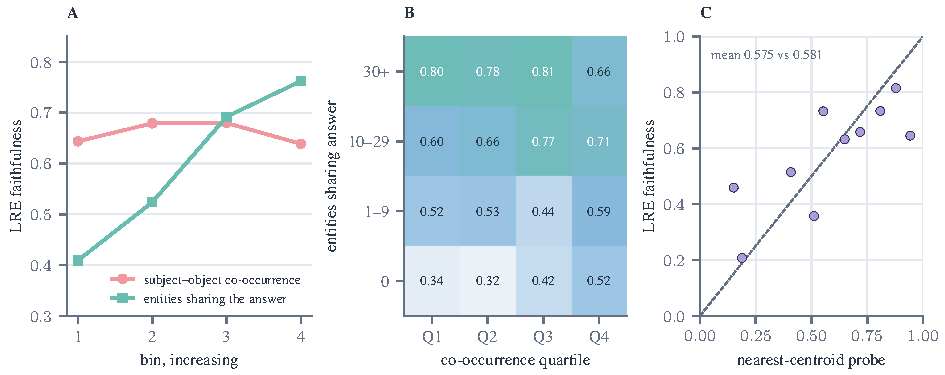
\includegraphics[width=1.0\textwidth]{lment_sharing.pdf}
  \caption{LRE faithfulness in LMEnt-1B increases when multiple subjects share
  the same answer (1,826 facts across ten relations). \textbf{A:} LRE
  faithfulness ($\phi_r$) across subject--object co-occurrence quartiles
  ($0.644$, $0.679$, $0.680$, $0.639$) and across bins of how many other
  subjects in the relation share the model's predicted answer ($0$: $0.409$;
  $1$--$9$: $0.524$; $10$--$29$: $0.692$; $30+$: $0.762$). \textbf{B:} Mean LRE
  faithfulness across the joint grid of answer sharing and co-occurrence
  quartiles (37 to 272 facts per cell). \textbf{C:} Per-relation LRE
  faithfulness versus a leave-one-out nearest-centroid classifier fit directly
  on the subject hidden states $h_s$ (dashed identity line).}
  \label{fig:lment-sharing}
\end{figure*}

\paragraph{Qualitative contrast within a single relation.}
The \emph{official language} relation illustrates how shared structure and raw
exposure can pull in opposite directions. The municipality of Lavertezzo appears
in only 13 linked training documents---nine placing it in the Italian-speaking
Swiss canton of Ticino, four mentioning the token \texttt{Italian}, and none
stating its official language---yet both LMEnt-1B and the LRE output
\texttt{Italian}, matching the many other Italian-speaking municipalities in the
relation (even when all Swiss and Italian examples are excluded from the LRE's
estimation prompt). Conversely, \texttt{Switzerland} co-occurs with its target
language 24{,}928 times across 106{,}201 documents; LMEnt-1B correctly outputs
\texttt{French} (shared by few entities in this relation), but the LRE outputs
\texttt{Swiss} and a linear probe on $h_s$ also fails. Shared class structure
supports linear relation decoding at low direct exposure, whereas heavy exposure
of an atypical pair does not.

\paragraph{Subject representations already cluster by answer before applying the LRE.}
Why does answer sharing predict LRE faithfulness? A leave-one-out
nearest-centroid classifier applied directly to the subject hidden states
$h_s$---without applying the relation Jacobian $W_r$---achieves $0.581$ accuracy
across the ten relations, slightly exceeding the LRE ($0.575$;
Figure~\ref{fig:lment-sharing}C). Moreover, of the 622 facts where the LRE
fails, a linear centroid probe on $h_s$ recovers 282 ($45\%$), because the mean
Jacobian $W_r$ is only weakly aligned with the empirical between-answer centroid
differences in $h_s$ (mean principal-angle cosine $0.341$, subspace overlap
$0.136$, versus $0.022$ for random directions in 2,048 dimensions). Thus, high
LRE faithfulness in LMEnt-1B primarily reflects that subjects sharing an object
already cluster together in $h_s$.

Because exposure, answer sharing, and entity prominence are confounded in
natural corpora, observational analysis of a pretrained model cannot isolate
their causal effects. We therefore turn to controlled synthetic pretraining
corpora that vary attribute structure and exposure frequency independently
(details of the LMEnt-1B evaluation are in Appendix~\ref{app:lment-frequency}).


\section{Experimental designs}
\label{sec:design}

Figure~\ref{fig:dataset-generation} illustrates our two synthetic dataset
constructions, both trained with standard causal next-token prediction
(full hyperparameters and architecture summaries are in
Appendix~\ref{app:training}).

\begin{figure*}[t]
\centering
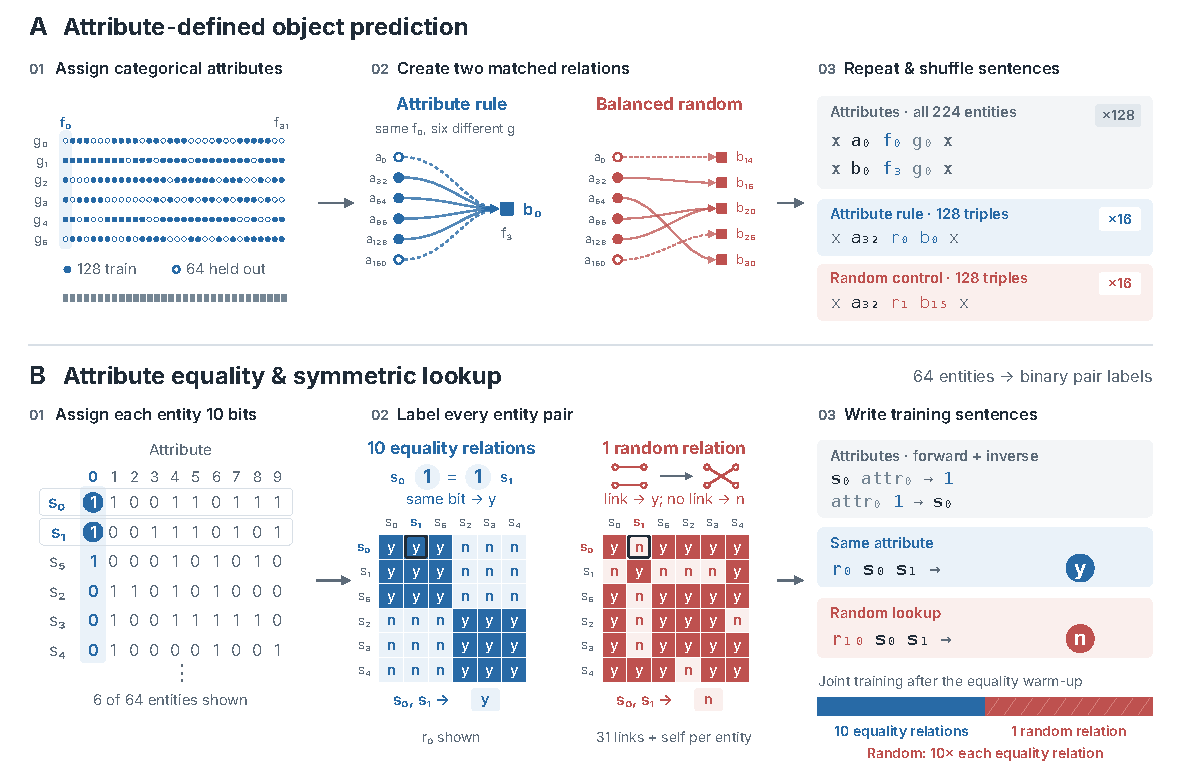
\includegraphics[width=1.0\textwidth]{synthetic_dataset_generation.pdf}
\caption{Synthetic dataset constructions for the two controlled experiments.
\textbf{A:} Categorical attributes $(f,g)$ define a fixed-shift object relation
$\Rsem$, paired with a frequency-matched random assignment $\Rrnd$. Filled and
hollow circles denote relation-trained (128) and held-out (64) subjects; all
subjects receive attribute supervision (shown for $F=16$). \textbf{B:} Ten
balanced binary attributes define ten symmetric attribute-equality relations
$r_1,\dots,r_{10}$, paired with a degree-matched symmetric random relation
$\Rrnd$ (six-entity excerpt from the 64-entity dataset; full specifications in
Appendix~\ref{app:training}).}
\label{fig:dataset-generation}
\end{figure*}

The two experiments test opposite ends of the frequency hypothesis and therefore
use complementary linear evaluation metrics and model shapes:
\begin{itemize}
  \item \textbf{Metrics:} Experiment~A tests whether low-exposure relation
  learning transfers to unseen subjects, so we fit an OLS linear probe on the
  128 trained subjects and report nearest-object classification accuracy on the
  64 held-out subjects. Experiment~B tests whether an arbitrary memorized table
  is stored with a linear embedding geometry; because a random lookup has no
  rule for unseen pairs, we fit OLS across all 64 memorized entities and report
  full-data multivariate $R^2$ (where $1$ indicates exact linear reconstruction
  and $0$ indicates no improvement over predicting the global mean target).
  \item \textbf{Model architectures:} In Experiment~A, a 1-layer causal
  transformer with residual width $d=64$ and untied input/output embeddings
  (84,288 parameters) suffices to learn the single-step attribute shift while
  allowing exact Jacobian and midpoint analysis of a single transformer layer.
  In Experiment~B, we use an 8-layer causal transformer with narrow residual
  width $d=20$ and tied input/output embeddings (41,760 parameters): keeping
  $d=20$ ensures that fitting $M_r\in\mathbb{R}^{20\times 20}$ plus bias
  $b_r\in\mathbb{R}^{20}$ (21 parameters per output coordinate) to 64 entities
  is strictly overdetermined ($21 \ll 64$), while the eight layers provide the
  nonlinear capacity required to memorize the $64\times 64$ random relation
  alongside the ten structured relations.
\end{itemize}

\subsection{Experiment A: Generalization from Shared Attributes}

Experiment~A contains 192 subjects $a_i$ covering all $32\times 6$ combinations
of two categorical attributes, $(f_{i\bmod 32},g_{\lfloor i/32\rfloor})$, and 32
objects $b_j$ whose $f$-attributes are shifted by a fixed offset. The structured
semantic relation maps each subject to the object with the matching shifted
$f$-attribute, $\Rsem(a_i)=b_{i\bmod32}$, while the random control
$\Rrnd(a_i)=b_{\rho(i)}$ uses a seed-dependent, attribute-independent balanced
assignment. For each of the 32 $f$-values, four subjects appear in relation
training and two are held out, yielding 128 trained and 64 held-out subjects per
relation. Every object is the target of four trained and two held-out subjects
under both $\Rsem$ and $\Rrnd$.

The training corpus consists of attribute sentences (describing the attributes
of every subject and object, each repeated $A=128$ times) and relation triples
(each of the 128 training triples per relation repeated $F\in\{1,4,16,64\}$
times; Appendix~\ref{app:training}). To test representation geometry, we fit an
OLS linear probe from each subject's input token embedding to its target
object's output token embedding on the 128 trained pairs, and evaluate top-1
cosine similarity accuracy over the 32 objects on the 64 held-out subjects
(chance is $1/32$).

\subsection{Experiment B: Memorization of Arbitrary Relations}

Experiment~B contains 64 entities characterized by ten balanced binary
attributes. Each attribute column has 32 zeros and 32 ones, all 64 entity
attribute vectors are distinct, and the centered attribute matrix has full rank
(10). Each structured relation $r_i$ ($i\in\{1,\dots,10\}$) is a binary
attribute-agreement relation that outputs \texttt{y} when two entities share
attribute $i$ and \texttt{n} otherwise:
\begin{equation}
  y_i(s,o)=\mathbb{1}[a_i(s)=a_i(o)].
  \label{eq:equality}
\end{equation}
Using binary attributes ensures that every structured relation partitions the 64
entities into two equal classes of 32 positive and 32 negative objects per
subject, creating a symmetric table that includes the diagonal and admits an
exact two-centroid linear target.

The eleventh relation, $\Rrnd$, is an arbitrary symmetric lookup table
constructed by sampling a simple 31-regular graph, randomizing edges with
degree-preserving swaps, and adding self-loops (rejecting any draw that matches
a structured table). This construction matches every structured relation's
symmetry, diagonal, degree (32 positives and 32 negatives per subject), and
class balance while removing attribute structure. Relation prompts take the form
\texttt{<bos> relation subject object} and predict \texttt{y} or \texttt{n}
across all $11\times64^2=45{,}056$ ordered pairs.

To ensure that the shared input/output token embeddings $e(s)\in\mathbb{R}^{20}$
encode the entity attributes through next-token prediction alone, the training
corpus includes both forward attribute examples (\texttt{<bos> subject attribute
0/1}) and inverse attribute examples (\texttt{<bos> attribute 0/1 subject}).
After an initial structured-only pretraining stage, joint training samples
$\Rrnd$ for 50\% of each relation batch and divides the remaining 50\% equally
across the ten structured relations (5\% each). Thus, $\Rrnd$ is sampled ten
times as often as any single structured relation during joint training (and
roughly five times as often over the complete curriculum;
Appendix~\ref{app:training}).

For each relation $r$, we define a subject's target representation as the
centroid of its 32 positive object token embeddings:
\begin{equation}
  c_r(s)=\frac{1}{32}\sum_{o:y_r(s,o)=1}e(o).
  \label{eq:centroid}
\end{equation}
We fit $c_r(s)\approx M_re(s)+b_r$ via OLS across all 64 entities and report
multivariate $R^2$. Representing each subject's target set by its positive-object
centroid summarizes all 32 positive objects in a single vector in
$\mathbb{R}^{20}$ and provides an exact analytic linear target for the binary
equality relations (whereas a linear classifier on concatenated $[e(s);e(o)]$
vectors would only test an additive pair score, which cannot represent binary
equality without bilinear interaction terms).

\section{Experiment A: Low exposure is compatible with linear representation geometry}
\label{sec:goal1-results}

We first evaluate Experiment~A to test whether shared attribute supervision
induces linear relation geometry at low direct exposure. At $F=16$ occurrences
per training triple, the structured relation $\Rsem$ reaches
\ExpOneSemanticTrained{} recall on trained subjects and \ExpOneSemanticHeldout{}
on held-out subjects, while the OLS linear probe transfers to held-out subjects
with $\ExpOneSemanticProbeStats$ accuracy (Table~\ref{tab:goal1}). In contrast,
the frequency-matched random relation $\Rrnd$ reaches only
\ExpOneRandomTrained{} trained recall and remains at chance ($1/32 \approx
0.031$) on both held-out recall and OLS transfer. Shared attribute structure
allows both the transformer and the linear probe to generalize to unseen
subjects, whereas matching exposure frequency on an arbitrary mapping yields
neither recall nor linear transfer.

\begin{table*}[t]
\centering
\small
\begin{tabular}{rcccccc}
\toprule
& \multicolumn{2}{c}{Held-out OLS accuracy}
& \multicolumn{2}{c}{Trained recall}
& \multicolumn{2}{c}{Held-out recall} \\
$F$ & $\Rsem$ & $\Rrnd$ & $\Rsem$ & $\Rrnd$ & $\Rsem$ & $\Rrnd$ \\
\midrule
1 & $1.000\pm0.000$ & $0.036\pm0.015$ & 0.029 & 0.010 & 0.016 & 0.010 \\
4 & $1.000\pm0.000$ & $0.016\pm0.013$ & 0.055 & 0.034 & 0.057 & 0.031 \\
16 & $0.990\pm0.007$ & $0.036\pm0.007$ & 0.672 & 0.167 & 0.635 & 0.031 \\
\bottomrule
\end{tabular}
\caption{Experiment~A results (mean $\pm$ SD over three seeds). $F$ is the
number of occurrences of each trained relation triple. OLS is fitted on the 128
trained subjects and evaluated on the 64 held-out subjects excluded from all
relation triples (chance is $1/32 \approx 0.031$).}
\label{tab:goal1}
\end{table*}

Crucially, this linear embedding geometry emerges before the model learns to
answer relation queries. At $F=1$, held-out OLS transfer is already $1.000$ even
though model recall on $\Rsem$ is near chance ($0.016$). Sweeping attribute
repetitions $A$ from 2 to 24 drives a sharp transition in held-out OLS accuracy
from \ExpOneTransitionLow{} to \ExpOneTransitionHigh{}
(Figure~\ref{fig:transition}, solid curve). A control model trained with
\emph{zero} relation triples ($F=0$, dashed curve) follows the exact same
trajectory, overlapping the $F=1$ curve throughout. Attribute supervision alone
therefore organizes the entity embeddings into a linearly decodable geometry,
even when the relation itself is never presented during training.

\begin{figure}[t]
  \centering
  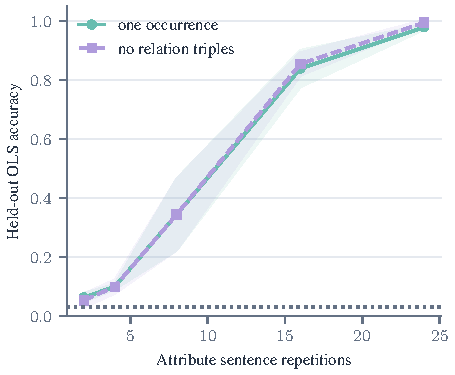
\includegraphics[width=1.0\linewidth]{linear_shift_transition.pdf}
  \caption{In Experiment~A, the $F=1$ curve (solid, one occurrence per semantic
  triple) and the $F=0$ control curve (dashed, zero relation triples in
  training) evolve identically as attribute repetitions $A$ increase from 2 to
  24. Attribute supervision alone drives the transition in held-out OLS accuracy
  (fitted on 128 subjects and evaluated on 64 held-out subjects; means $\pm$ 1
  SD over three seeds).}
  \label{fig:transition}
\end{figure}

Next, we test whether the 1-layer transformer's \emph{executed forward pass}
$h(x)$ at $F=16$ is itself a linear (plus offset) function of the subject
embedding $x$ when holding the relation token fixed (full sublayer breakdown in
Appendix~\ref{app:goal1-extra}). If a continuous mapping $h(x)$ had the exact
form $h(x)=Mx+b$, it would satisfy two identities: (i) its output at the
midpoint between any two inputs $(x_i+x_j)/2$ would equal the midpoint of their
outputs $(h(x_i)+h(x_j))/2$, and (ii) its input--output Jacobian matrix
$J(x)=\partial h/\partial x$ would be constant across all inputs. We quantify
relative violations of these two conditions via \emph{midpoint defect}
$D_{\mathrm{mid}}$ and \emph{Jacobian dispersion} $D_J$ (both $0$ when
$h(x)=Mx+b$; formal definitions in Appendix~\ref{app:metrics}), alongside the
cross-validated $R^2$ of a linear regression fitted directly to the forward map
$h(x)$. For the complete subject-to-logit forward pass, a linear fit captures
most of the output variance ($R^2=\ExpOneAffine$), yet both the midpoint defect
($D_{\mathrm{mid}}=\ExpOneMidpoint$) and Jacobian dispersion
($D_J=\ExpOneJacobian$, or $\ExpOneTangent$ restricted to the empirical
subject-difference subspace) are substantial. Thus, while the forward mapping is
well approximated by a linear function on the training distribution, the
executed computation is genuinely nonlinear.

Activation patching shows how this nonlinear forward pass uses the attribute
representations (details in Appendix~\ref{app:goal1-extra}). First, a
nearest-centroid classifier trained on the 128 relation-training embeddings
recovers the $f$-attribute class of all 64 held-out subject embeddings with
100\% accuracy. During inference, patching the attention heads' value vectors
from a clean subject into a corrupted prompt recovers $\ExpOneValuePatch$ of the
target-logit margin, whereas patching attention weights recovers only
$\ExpOnePatternPatch$, and replacing all attention head outputs with their
training-subject mean reduces accuracy from $\ExpOneHeadsPresent$ to chance.
Patching at the relation-token position shows that the MLP layer combines the
attended subject representation with the relation token ($\ExpOneRelationPatch$
recovery) across a distributed population of MLP neurons (retaining only the top
32 neurons by causal effect recovers $\ExpOneTopOnly$ of the subject-specific
margin, while ablating those 32 still leaves $\ExpOneTopAblated$). In short,
attention copies the subject's $f$-attribute representation to the final
position, where the MLP maps it nonlinearly to the shifted target object.

\section{Experiment B: High exposure is compatible with nonlinear representation geometry}
\label{sec:goal2-results}

In Experiment~B, the eight-layer transformer learns both the ten structured
attribute-equality relations and the heavily sampled random relation $\Rrnd$
almost perfectly. Across all three seeds, attribute accuracy is 100\%, relation
accuracies range from 99.98\% to 100\% (Table~\ref{tab:goal2}), and minimum
prediction symmetry $(y(s,o)=y(o,s))$ across all eleven relations is 99.95\%.
Memorizing the random lookup table therefore does not interfere with learning
the structured relations.

\begin{table}[t]
\centering
\small
\setlength{\tabcolsep}{3pt}
\begin{tabular}{lrrrr}
\toprule
 & \multicolumn{2}{c}{Accuracy (\%)} & \multicolumn{2}{c}{OLS $R^2$} \\
Seed & Min. struct. & Random & Min. struct. & Random \\
\midrule
19 & 99.98 & 100.00 & 0.996 & 0.384 \\
31 & 99.98 & 99.98 & 0.995 & 0.401 \\
47 & 99.98 & 99.98 & 0.995 & 0.340 \\
\midrule
Mean & 99.98 & 99.98 & 0.995 & 0.375 \\
\bottomrule
\end{tabular}
\caption{Complete-table accuracy and full-data OLS $R^2$ in Experiment~B.
Structured columns report the minimum across the ten attribute-equality
relations within each seed. OLS maps the 20-dimensional subject token embeddings
to positive-object centroids across all 64 entities.}
\label{tab:goal2}
\end{table}

Despite identical behavioral accuracy, the underlying token-embedding geometries
differ sharply. Across the 30 structured fits (10 relations $\times$ 3 seeds),
mean full-data $R^2$ is 0.997 and every fit exceeds 0.994. For the random
relation $\Rrnd$---despite being sampled ten times as often as each structured
relation during joint training---full-data $R^2$ ranges from 0.340 to 0.401
(mean \ExpTwoRandomRsq{}), leaving over 60\% of the target centroid variance
unexplained.

Why do the structured relations admit an exact linear fit? Writing
$b_i(s)=2a_i(s)-1\in\{-1,+1\}$ for attribute $i$ and letting $\mu_i^+$ and
$\mu_i^-$ denote the token-embedding centroids of entities with $a_i=1$ and
$a_i=0$, the positive-object centroid for relation $r_i$ is an exact linear
function of $b_i(s)$ (plus a constant offset):
\begin{equation}
  c_i(s)=\mu_i^-+\frac{b_i(s)+1}{2}(\mu_i^+-\mu_i^-).
  \label{eq:structured-affine}
\end{equation}
Because the inverse attribute examples align the coordinates of $e(s)$ with the
binary attributes $b_i(s)$, a single linear regression $M_ie(s)+b_i$ recovers
$c_i(s)$ with $R^2 > 0.994$. The random graph $\Rrnd$ matches every structured
relation's degree, symmetry, and class balance, but lacks any shared attribute
rule to align its positive-object centroids with $e(s)$.

In fact, most of the random relation's observed $R^2=\ExpTwoRandomRsq{}$ simply
reflects the baseline degrees of freedom of fitting 21 parameters (20 input
dimensions plus an intercept) to 64 entities: simultaneously permuting entity
rows and columns yields a null mean $R^2$ of $\ExpTwoNullMean{}$, placing the
three seeds at the 94.8th, 98.0th, and 49.2nd null percentiles (four-fold
cross-validated $R^2$ is correspondingly negative;
Appendix~\ref{app:goal2-extra}). Thus, even under heavy repetition, the
memorized random relation remains near the random-permutation floor of linear
decodability.


\begin{figure*}[t]
  \centering
  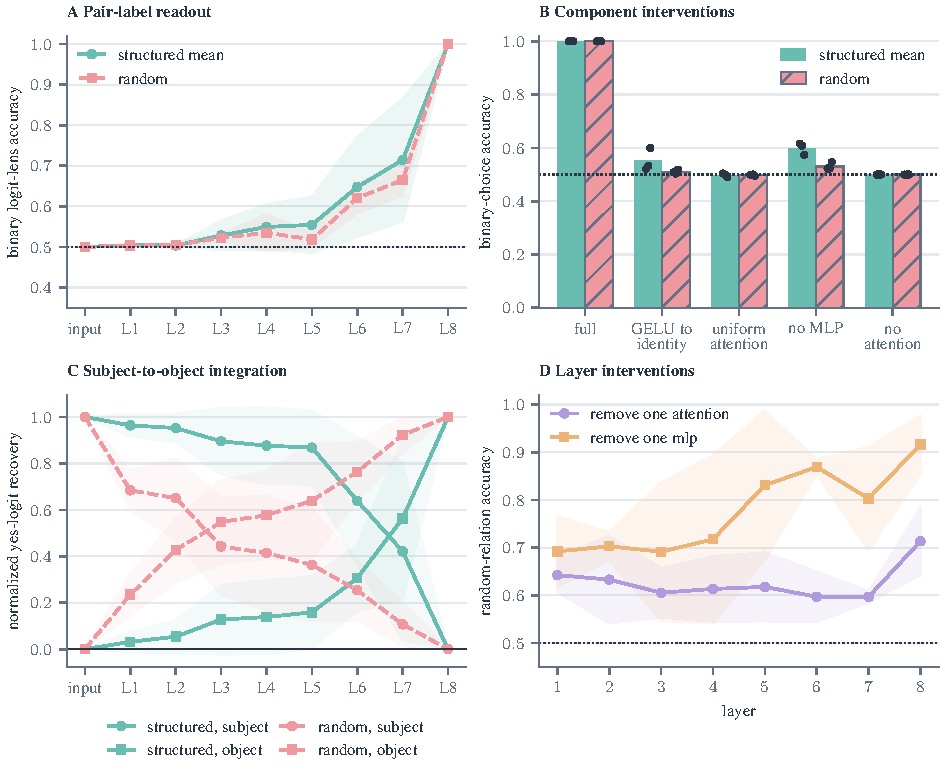
\includegraphics[width=1.0\textwidth]{goal2_raw_transformer_mechanism.pdf}
  \caption{In Experiment~B, the memorized random relation relies on distributed
  nonlinear computation across the eight transformer layers (means $\pm$ 1 SD
  over three seeds). \textbf{A:} A layerwise logit lens tracks when the random
  answer becomes linearly readable across the eight layers. \textbf{B:} Global
  interventions on GELU activations, attention routing, MLP outputs, or
  attention outputs degrade accuracy on both structured and random relations.
  \textbf{C:} Residual-stream patching shows relational information shifting
  from the subject position to the object position across layers. \textbf{D:}
  Ablating any single attention or MLP sublayer impairs random-relation recall,
  showing that the lookup is distributed across layers.}
  \label{fig:goal2-mechanism}
\end{figure*}

\section{The memorized random lookup uses distributed nonlinear computation}
\label{sec:mechanism}

How does the eight-layer transformer in Experiment~B achieve 99.98\% accuracy on
$\Rrnd$ when a linear regression on the embeddings explains only 37.5\% of its
target centroid variance? We apply causal interventions and layerwise probing to
identify how the forward pass computes the memorized lookup
(Figure~\ref{fig:goal2-mechanism}).

With trained weights fixed, replacing GELU activations with the identity
function reduces random-relation accuracy from nearly 100\% to 51\%. Making
attention weights uniform or ablating all attention or MLP outputs likewise
reduces accuracy to near chance (50\%; Figure~\ref{fig:goal2-mechanism}B). The
memorized lookup therefore depends on nonlinear MLP activations and
content-dependent attention routing.

A layerwise logit lens shows that the correct yes/no answer for $\Rrnd$ becomes
linearly decodable from the residual stream only in the final transformer layer
(Figure~\ref{fig:goal2-mechanism}A). Nevertheless, ablating any single attention
or MLP sublayer in earlier layers degrades accuracy
(Figure~\ref{fig:goal2-mechanism}D), showing that intermediate layers
incrementally construct the lookup representation.

Residual-stream patching across layers tracks how information moves between
token positions (Figure~\ref{fig:goal2-mechanism}C; metric details in
Appendix~\ref{app:metrics}). Patching the clean subject representation into a
corrupted prompt recovers the answer margin in early layers, whereas patching
the object position recovers the margin in later layers, consistent with
attention routing subject information to the final object position where the
yes/no prediction is emitted. Because global component ablations impair both
structured and random relations (Figure~\ref{fig:goal2-mechanism}B), both rely
on nonlinear forward computation; what distinguishes them is whether the
underlying entity embeddings organize into a linearly decodable geometry.



\section{Discussion}

\paragraph{Shared structure drives linear relational decodability.}
Our two synthetic experiments decouple exposure frequency from relational
structure and reverse the naive frequency association in both directions. In
Experiment~A, shared attribute supervision induces a linearly decodable
embedding geometry before the model even recalls the relation triples. In
Experiment~B, heavy repetition allows an eight-layer transformer to memorize an
arbitrary relation to 99.98\% accuracy while its token-embedding $R^2$ remains
near the permutation floor. In natural-language pretraining corpora, exposure
frequency is naturally correlated with attribute sharing, entity prominence, and
paraphrase diversity. Consistent with our synthetic results, our LMEnt-1B
analysis shows that within natural relations, LRE faithfulness tracks how many
subjects share an answer rather than how often a subject--object pair co-occurs
in the corpus.

\paragraph{Linear decodability depends on the chosen representation.}
In Experiment~B, the memorized random relation has a poor linear fit in the
shared input/output token embedding space compared with the structured
controls. More accurate linear readouts for arbitrary relations may emerge in
later hidden layers after nonlinear attention and MLP layers have routed
subject and object information (as shown by our layerwise logit lens in
Figure~\ref{fig:goal2-mechanism}A).

\paragraph{Representation geometry and executed computation are distinct.}
In Experiment~A, token embeddings support near-perfect held-out OLS transfer,
yet midpoint defects and Jacobian dispersion show that the executed 1-layer
forward pass is nonlinear. In Experiment~B, both structured and random relations
depend causally on GELU activations and content-dependent attention routing, yet
only the structured relations organize the token embeddings into a linearly
decodable centroid geometry. Linear probe performance on static representations
should therefore not be conflated with linearity of the circuit executing the
forward pass.

\section{Conclusion}

Exposure frequency alone does not determine whether a transformer encodes a
relation with a linear representation geometry. Shared attribute supervision can
organize entity embeddings into a linearly decodable subspace even at minimal
relation exposure, whereas a heavily repeated arbitrary relation can be
memorized nearly perfectly without inducing a linear relational representation
in token-embedding space. Likewise, in pretrained LMEnt-1B, LRE faithfulness
within relations is predicted by answer sharing rather than document
co-occurrence frequency. Claims about relational linearity should therefore
specify behavioral accuracy, which representations are connected by the linear
probe, and whether the evidence tests representation decodability or the
executed forward computation.

\section*{Limitations}

\paragraph{Memorization of a fixed graph versus open-ended generalization.}
In Experiment~B, $\Rrnd$ is a fixed 64-entity random graph with no latent rule
relating unseen pairs. This design isolates whether repetition alone forces a
known lookup table into a linear embedding representation, but it does not model
out-of-distribution generalization to new entities.

\paragraph{Curriculum and model scope.}
In Experiment~B, the inverse attribute examples (\texttt{<bos> attribute 0/1
subject}) explicitly encourage the tied token embeddings to organize by
attribute under the next-token prediction loss. Because we did not ablate these
inverse examples or sweep alternative architectures after selecting our
experimental configuration, the near-perfect token-embedding $R^2$ on structured
relations is conditional on this training curriculum. Similarly, our
natural-language analysis evaluates a single pretrained checkpoint (LMEnt-1B)
using observational document counts; performing causal curriculum interventions
during large-scale natural-language pretraining remains an important direction
for future work.

\paragraph{Selected exposure regimes rather than full response surfaces.}
Our synthetic experiments establish clear counterexamples at selected exposure
ratios across three random seeds, showing that low exposure can coexist with
linear representation geometry and high relative exposure can coexist with
nonlinear representation geometry.
Notice also that occurrence counts are defined within each synthetic task and
are not directly comparable across the two vocabulary sizes and optimization
schedules. Mapping the full joint response surface across broader architectures,
embedding dimensions, and relation arities requires wider hyperparameter sweeps.

\section*{Acknowledgements}
% Same two DFG grants as the relational-decoding preprint in jlens.
This work was supported by the German Research Foundation (DFG) under
grants SCHU~2246/14-1 and GU~798/29-1 (UKP-SQuARE project).
We gratefully acknowledge support from Google through a generous GCP research grant.

\subsubsection*{AI use statement}
Generative AI tools were used to help design and critique the synthetic
experiments, implement and edit software, generate synthetic data and plots,
analyze and interpret experimental outputs, search and summarize literature, and
draft and edit this manuscript. The authors inspected the generated code, ran the
reported experiments and automated tests, checked numerical claims against
experimental results, reviewed the cited primary sources, and revised the
resulting text. The authors take responsibility for the paper's claims and
contents.

\bibliography{references}

\clearpage
\appendix

\section{Reproducibility statement}
\label{app:reproducibility}

We provide a Docker pipeline for training and evaluating both synthetic
experiments, aggregating the archived LMEnt frequency observations, and generating
the associated figures, tables, and paper PDF. With the images built, two fresh
runs each completed in under one hour on consumer-grade hardware: a Ryzen 9
7950X3D CPU and one RTX 4090 GPU. The runs reproduced all recorded synthetic
numerical results and checkpoint tensors exactly on this setup. The pipeline
uses saved LMEnt observations rather than rerunning pretrained-model inference.

\paragraph{Implementation and numerical settings.}
Training uses PyTorch 2.12.0 with CUDA 13.0 \citep{paszke2019pytorch}; linear regression
fits use scikit-learn 1.9.0 \citep{pedregosa2011scikit}. The Docker environment
pins dependencies and enables deterministic computation. OLS includes an
intercept and no regularization. Experiment~B uses double precision and four
shuffled cross-validation folds with the experiment seed. AdamW uses
$\beta_1=0.9$, $\beta_2=0.999$, and $\epsilon=10^{-8}$; remaining training
settings appear in Appendix~\ref{app:training}. Results aggregate seeds 19, 31,
and 47. Experiment~A numerical summaries use population standard deviations;
its transition plot and Experiment~B use sample standard deviations. LMEnt
rank correlations use average ranks for ties and quartiles use linear
interpolation.

\paragraph{Data and model scope.}
The synthetic corpora contain generated categorical symbols; construction and
splits appear in Appendix~\ref{app:training}. The natural-language analysis uses
LMEnt-1B-1E at step 109,672 \citep{gottesman2025lment}, pretrained on English
Wikipedia, and 5,388 evaluated facts across 58 relations
(Appendix~\ref{app:lment-frequency}). These observations retain names and
Wikidata identifiers, including 2,529 rows in person relations. Model predictions
are research outputs, not verified biographical information. No human
participants or external annotators were recruited.


\section{Complete training protocols}
\label{app:training}

\begin{table*}[t]
\centering
\small
\begin{tabular}{lll}
\toprule
 & Experiment A & Experiment B \\
\midrule
Question & low-exposure relational linearity & frequent nonlinear relation \\
Entities & 192 subjects, 32 objects & 64 entities \\
Structure & 2 categorical attributes & 10 balanced binary attributes \\
Relations & semantic + matched random & 10 equality + symmetric random \\
Model & 1 layer, width 64 & 8 layers, width 20 \\
Parameters & 84,288 & 41,760 \\
Embedding setup & untied, trainable & tied, trainable \\
Primary linearity test & held-out OLS accuracy & full-data OLS $R^2$ \\
\bottomrule
\end{tabular}
\caption{Summary of experimental designs for Experiment~A and Experiment~B.}
\label{tab:design}
\end{table*}

\subsection{Experiment A}

The causal transformer has one transformer layer, residual width 64, four
attention heads, context length 8, and untied input and output token embeddings.
All 84,288 parameters are initialized from $\mathcal{N}(0,0.02^2)$. Training
uses AdamW with learning rate $10^{-3}$, five warmup steps, no weight decay, and
gradient clipping at 1.

Every training sentence contains five tokens. Attribute sentences have the form
\texttt{x subject f-attribute g-attribute x}, and relation sentences have the
form \texttt{x subject relation object x}. The vocabulary contains 265 tokens:
one separator, two relations, 192 subjects, 32 objects, 32 $f$ values, and six
$g$ values. Object $b_j$ has attributes $(f_{(j+3)\bmod32},g_0)$, while the
semantic target of $a_i$ is $b_{i\bmod32}$, linking each subject to its target
object through a constant shift in $f$-attribute values.

For each $f$ value, a seed-dependent split assigns four subjects to relation
training and two to held-out evaluation. The random target assignment is
balanced within both groups so that every object is the target of four training
subjects and two held-out subjects under either relation, matching relation,
subject, and object-target frequencies exactly.

At $F=16$, the corpus contains 28,672 attribute sentences and 4,096 relation
sentences (32,768 total). Training runs for one complete shuffled pass through
the corpus with unweighted next-token cross-entropy at every position. At batch
size 64, this corresponds to 452 optimizer updates for $F=1$, 464 for $F=4$, 512
for $F=16$, and 704 for $F=64$. Data splits, model initialization, and shuffle
order vary with the random seed.

\subsection{Experiment B}

The vocabulary contains 90 tokens: one beginning-of-sequence token, 64 entities,
ten attributes, eleven relations, and output symbols \texttt{0}, \texttt{1},
\texttt{n}, and \texttt{y}. The decoder-only transformer has eight pre-LayerNorm
transformer layers, residual width 20, four attention heads (head width
5), GELU MLP width 80, and context length 4. Token embeddings, position
embeddings, all eight layers, final LayerNorm, and the tied output projection
are trained jointly (41,760 parameters total).

Training uses AdamW with no weight decay, gradient clipping at 1, and a 100-step
linear warmup. Relation batches contain 1,024 examples, and attribute batches
sample 640 examples with replacement. Every relation uses a 1:9
positive-to-negative sampling ratio with positive labels weighted by 9; forward
attribute loss has weight 1 and inverse attribute loss has weight 4. Structured
pretraining adapts relation sampling to prediction errors and runs for 6,000
steps at learning rate $10^{-3}$ (evaluated every 500 steps). Joint training
samples $\Rrnd$ for half of each relation batch and splits the remaining half
uniformly across the ten structured relations for up to 12,000 steps at
$10^{-3}$ (evaluated every 500 steps for seed 19 and every 1,000 steps for seeds
31 and 47), followed by up to 8,000 continuation steps at $3\times10^{-4}$
(evaluated every 200 steps) and, for seeds 19 and 31, up to 3,000 steps at
$10^{-4}$ (evaluated every 100 steps), resetting optimizer and RNG states between
stages. Joint stages stop at the first evaluated checkpoint satisfying all
behavioral, symmetry, and geometry criteria: attribute accuracy, every relation
accuracy, and every prediction-symmetry agreement at least $0.995$, every
structured full-data $R^2$ at least $0.95$, and random full-data $R^2$ below
$0.50$. For all three seeds, structured pretraining completes 6,000 steps, the
first joint stage completes 12,000 steps, and the first continuation stage stops
after 200 steps (with seeds 19 and 31 completing 100 steps in the final stage).

\section{Additional Experiment A results}
\label{app:goal1-extra}

\begin{table*}[t]
\centering
\scriptsize
\setlength{\tabcolsep}{3.6pt}
\begin{tabular}{lccccc}
\toprule
Map & Linear $R^2$ & Relative error & Linear decision & Midpoint defect & Jacobian dispersion \\
\midrule
Attention core & $0.993\pm0.002$ & $0.080\pm0.012$ & $0.747\pm0.069$ & $0.035\pm0.007$ & $0.085\pm0.013$ \\
Attention sublayer & $0.983\pm0.004$ & $0.129\pm0.015$ & $0.750\pm0.066$ & $0.273\pm0.010$ & $0.179\pm0.005$ \\
MLP core & $0.982\pm0.004$ & $0.133\pm0.013$ & $0.747\pm0.068$ & $0.095\pm0.005$ & $0.137\pm0.007$ \\
MLP sublayer & $0.974\pm0.006$ & $0.160\pm0.017$ & $0.758\pm0.057$ & $0.247\pm0.027$ & $0.172\pm0.009$ \\
Readout & $0.993\pm0.003$ & $0.081\pm0.017$ & $0.760\pm0.060$ & $0.199\pm0.004$ & $0.228\pm0.007$ \\
Full lookup & $0.965\pm0.010$ & $0.185\pm0.027$ & $0.750\pm0.056$ & $0.352\pm0.011$ & $0.281\pm0.013$ \\
\bottomrule
\end{tabular}
\caption{Sublayer and full-lookup linearity diagnostics for $\Rsem$ at $F=16$ in
Experiment~A (four target-stratified folds; mean $\pm$ SD over three seeds). An
exact first-order linear relation transformation has zero midpoint defect and zero Jacobian
dispersion. The linear decision column reports top-1 object accuracy when the
sublayer's output is replaced by its cross-validated linear regression approximation.}
\label{tab:goal1-transformations}
\end{table*}

At $F=64$, the random relation $\Rrnd$ reaches $1.000$ recall on trained
subjects, confirming that the 1-layer architecture can memorize the arbitrary
training pairs given sufficient exposure, while remaining at chance ($1/32$) on
held-out subjects and held-out OLS transfer.

For the causal patching experiments in Experiment~A, we measure target-logit
margin recovery, defined as the patched-minus-corrupted target logit change
divided by the clean-minus-corrupted change (aggregated across prompts before
division). For $\Rsem$ at $F=16$, patching subject-derived attention value
vectors recovers $\ExpOneValuePatch$ of the clean margin, whereas patching
attention weights recovers $\ExpOnePatternPatch$. Patching all MLP activations
at the relation-token position recovers $\ExpOneRelationPatch$ of the
relation-specific margin. Retaining only the 32 MLP neurons with the largest
individual effects recovers $\ExpOneTopOnly$ of the subject-specific margin,
while ablating those 32 neurons still leaves $\ExpOneTopAblated$, indicating a
distributed MLP readout.

\section{Additional Experiment B results}
\label{app:goal2-extra}

\begin{table*}[t]
\centering
\scriptsize
\setlength{\tabcolsep}{2.8pt}
\begin{tabular}{lrrrrrrr}
\toprule
Seed & Attribute & Min. struct. & Random & Min. symmetry & Min. struct. $R^2$ & Random $R^2$ & Random CV $R^2$ \\
\midrule
19 & 1.00000 & 0.99976 & 1.00000 & 0.99951 & 0.99569 & 0.38385 & -0.65023 \\
31 & 1.00000 & 0.99976 & 0.99976 & 0.99951 & 0.99529 & 0.40066 & -0.76091 \\
47 & 1.00000 & 0.99976 & 0.99976 & 0.99951 & 0.99485 & 0.34028 & -0.72857 \\
\midrule
Mean & 1.00000 & 0.99976 & 0.99984 & 0.99951 & 0.99527 & 0.37493 & -0.71324 \\
\bottomrule
\end{tabular}
\caption{Complete behavioral accuracy, prediction symmetry, and token-embedding
OLS $R^2$ (full-data and four-fold cross-validated) across seeds in
Experiment~B.}
\label{tab:goal2-complete}
\end{table*}

\begin{figure*}[t]
  \centering
  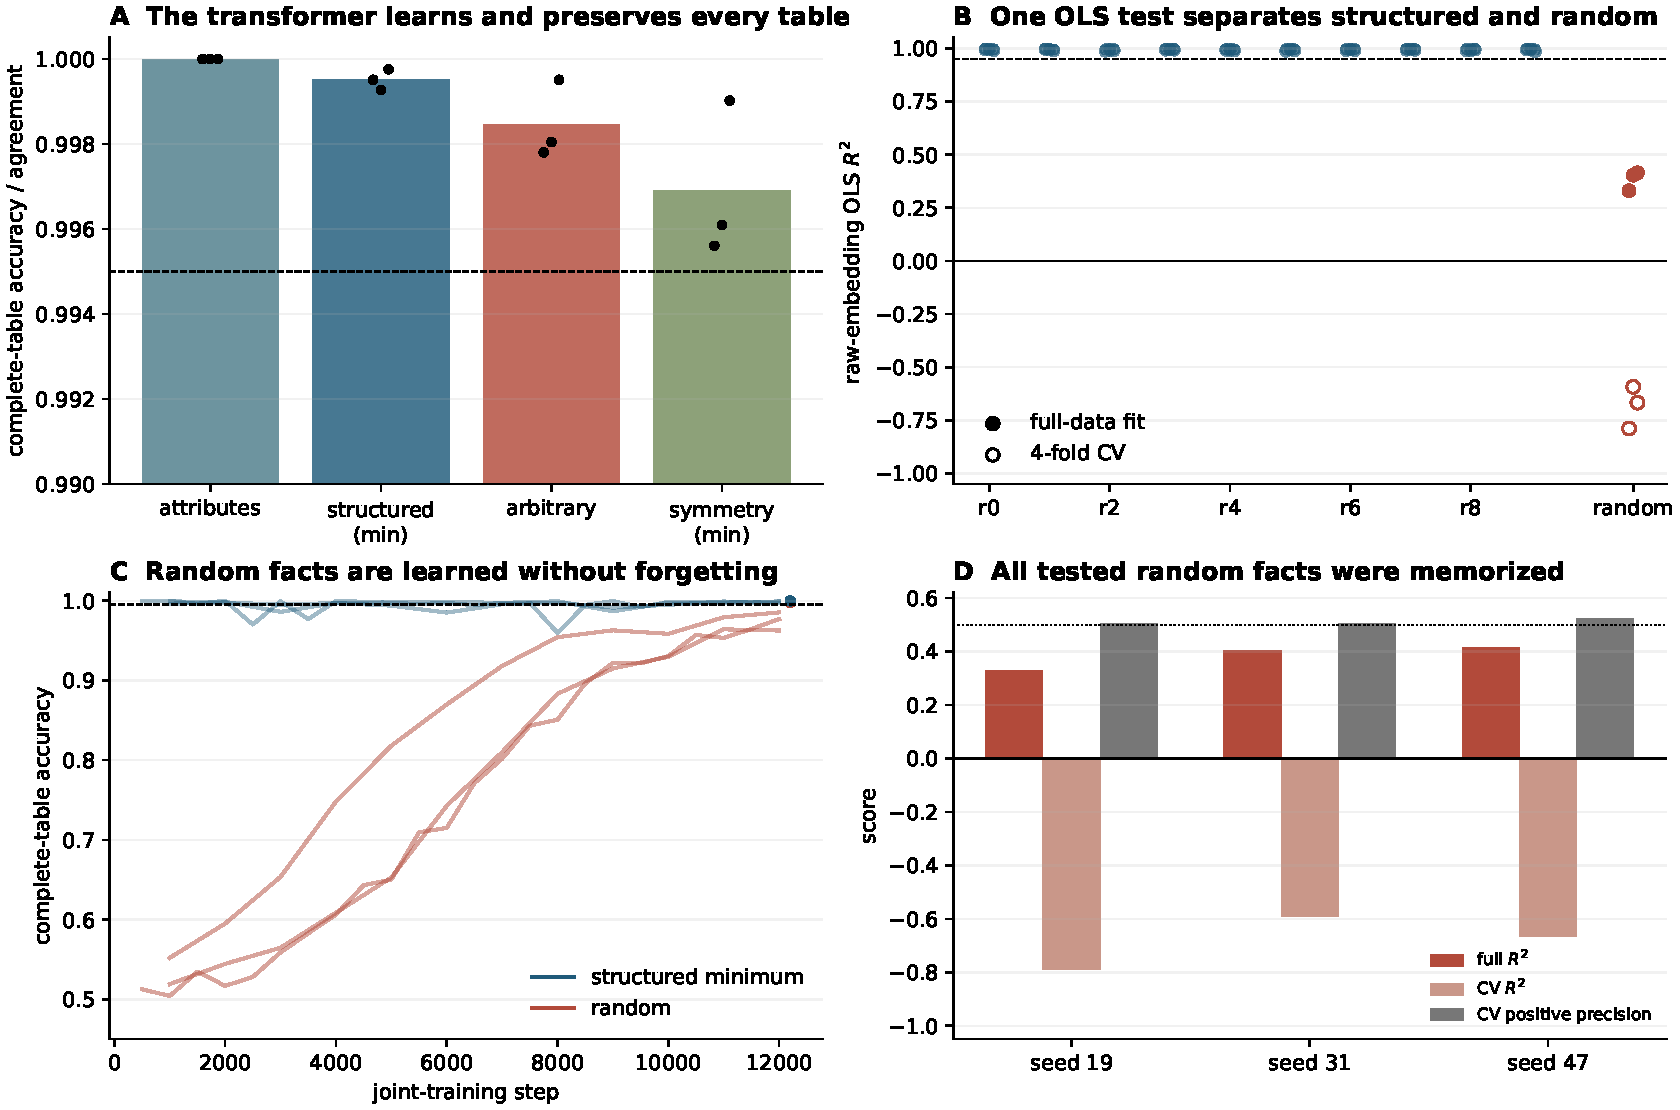
\includegraphics[width=1.0\textwidth]{goal2_raw_transformer_results.pdf}
  \caption{Training trajectories and final linear-fit diagnostics for
  Experiment~B. Filled OLS markers show full-data $R^2$ across all 64 entities;
  open markers show four-fold cross-validated $R^2$. Dashed horizontal lines mark
  the stopping thresholds.}
  \label{fig:goal2-complete}
\end{figure*}

Under the global component interventions shown in
Figure~\ref{fig:goal2-mechanism}B, mean accuracy on the ten structured relations
is $\ExpTwoStructuredFullPrecise$ in the unablated model,
$\ExpTwoStructuredGeluPrecise$ when replacing GELU with the identity function,
$\ExpTwoStructuredUniformPrecise$ under uniform attention weights,
$\ExpTwoStructuredNoMlpPrecise$ when removing all MLP outputs, and
$\ExpTwoStructuredNoAttentionPrecise$ when removing all attention outputs. The
corresponding accuracies on the random relation $\Rrnd$ are
$\ExpTwoRandomFullPrecise$, $\ExpTwoRandomGeluPrecise$,
$\ExpTwoRandomUniformPrecise$, $\ExpTwoRandomNoMlpPrecise$, and
$\ExpTwoRandomNoAttentionPrecise$.

\section{Metric details}
\label{app:metrics}

For an Experiment~A sublayer or full-lookup mapping $h$, let $z_i=h(x_i)$. The
normalized midpoint defect is
\begin{equation}
  D_{\mathrm{mid}}=
  \frac{\left(\sum_{(i,j)\in\mathcal P}
  \left\|h\left(\tfrac{x_i+x_j}{2}\right)
  -\tfrac{z_i+z_j}{2}\right\|_2^2\right)^{1/2}}
  {\left(\sum_{(i,j)\in\mathcal P}
  \left\|\tfrac{z_i-z_j}{2}\right\|_2^2\right)^{1/2}}.
\end{equation}
The diagnostic fold contains one trained subject for each of the 32 target
objects, and $\mathcal P$ contains all $\binom{32}{2}=496$ unordered pairs with
distinct targets. Each midpoint $h((x_i+x_j)/2)$ is evaluated through the
continuous residual-stream extension of the trained network while holding the
separator and relation tokens fixed.

Let $J_i=\partial h/\partial x\vert_{x_i}$ denote the exact Jacobian at subject
$x_i$ (computed via automatic differentiation) and $\bar J=32^{-1}\sum_{i=1}^{32} J_i$
denote the fold mean. Relative Jacobian dispersion is
\begin{equation}
  D_J=\frac{\left(\sum_i\|J_i-\bar J\|_F^2\right)^{1/2}}
  {\left(\sum_i\|J_i\|_F^2\right)^{1/2}}.
\end{equation}
Tangent-subspace dispersion applies the same formula to $J_iQ$, where the
columns of $Q$ form an orthonormal basis for the empirical subject-difference
subspace (retaining singular values above $10^{-6}$ of the maximum). Both
diagnostics are evaluated on the first target-stratified fold for each of the
three training seeds.

For Experiment~B, full-data OLS minimizes
\begin{equation}
  (\widehat M_r,\widehat b_r)=\arg\min_{M,b}\sum_{s=0}^{63}
  \left\|c_r(s)-Me(s)-b\right\|_2^2,
\end{equation}
and the multivariate coefficient of determination is
\begin{equation}
  R_r^2=1-
  \frac{\sum_s\|c_r(s)-\widehat M_re(s)-\widehat b_r\|_2^2}
       {\sum_s\|c_r(s)-\overline c_r\|_2^2},
\end{equation}
pooling all 20 output coordinates in the numerator and denominator (with
relative reconstruction error $\sqrt{1-R_r^2}$). Because ordinary least squares
is the unconstrained minimizer of this training-set residual sum of squares,
adding $\ell_2$ (ridge) regularization or rank constraints cannot increase
full-data $R_r^2$.

For residual-stream patching in Experiment~B, a clean prompt uses a correctly
classified positive subject ($y_r(s^+,o)=1$) and a corrupted prompt uses a
correctly classified negative subject ($y_r(s^-,o)=0$) while holding the
relation $r$ and object $o$ fixed. For the binary answer logit margin
$m=\ell_{\texttt{y}}-\ell_{\texttt{n}}$, recovery after patching layer boundary
$k$ is
\begin{equation}
  \operatorname{recovery}_k=
  \frac{\sum_j(m^{(j)}_{\mathrm{patched},k}-m^{(j)}_{\mathrm{corrupt}})}
       {\sum_j(m^{(j)}_{\mathrm{clean}}-m^{(j)}_{\mathrm{corrupt}})},
\end{equation}
where patching replaces either the subject-position or object-position hidden
state in the corrupted run with its clean counterpart and executes the remaining
transformer layers.

\section{Pretrained-model aggregation details}
\label{app:lment-frequency}

The LMEnt-1B evaluation covers 5,388 facts across 58 of the dataset's 60
relation types (two relations lack enough accepted examples for the
eight-demonstration estimation protocol). The model has 18 OLMo2 transformer
layers and residual width 2,048. Overall first-token decoder agreement
(faithfulness) is $51.1\%$ when weighting facts equally and $54.4\%$ when
weighting relations equally.

Subject frequency counts distinct corpus documents (chunks) linked to a
subject's Wikidata identifier. Subject--object frequency counts subject-linked
documents that also contain the gold object label, matched case-insensitively at
word boundaries (including recorded country and continent demonym aliases), while
subject--relation frequency requires a recorded lexical relation cue. Because
co-occurrences and lexical cues need not express the target fact---and zero
document matches do not guarantee zero training exposure---these counts serve as
observational proxies for pretraining exposure.

Following the source protocol, we use random seed 42 and an
object-coverage-balanced ordering to select eight LRE estimation examples per
relation, which are excluded from evaluation and used as in-context
demonstrations in evaluation prompts. An example is retained when the model's
top-1 predicted token (stripped of whitespace and lowercased) matches a nonempty
prefix of the gold object label. Candidate subject representations are extracted
from residual-stream states after layers $\{0,3,6,9,12,15\}$ (0-indexed). The
archived scale sweep over $\beta\in\{1,2,3,4,5,6,8,10\}$ maximizes macro-average
best-layer faithfulness across relations, selecting $\beta=4$ (note that layer
and scale selection use the evaluation split rather than a separate validation
split).

At the relation level, correlating $\log(1+\bar f_r)$ (where $\bar f_r$ is the
mean subject--object document count across evaluated facts in relation $r$) with
relation faithfulness yields a Pearson correlation of $-0.08$ across all 58
relations, $0.10$ across the 48 relations with more than one distinct predicted
answer token, and $0.21$ across the 33 relations that also have at least 20
evaluated facts (or $0.10$ using $\log\bar f_r$ after excluding zero-frequency
relations). Unlike \citet{merullo2025frequency}, who evaluate intervention
causality against tokenized sequence counts in OLMo-7B with per-relation scale
selection, our LMEnt-1B analysis evaluates observational decoder faithfulness
against entity-linked document counts.

Within each relation and frequency axis, let $q_{.25}$ and $q_{.75}$ denote the
empirical 25th and 75th percentiles (computed via linear interpolation), and
define the lower and upper quartile groups as $f_i\leq q_{.25}$ and $f_i\geq
q_{.75}$ (retaining all tied observations and requiring $q_{.25}<q_{.75}$ so
that the groups are disjoint). The upper-minus-lower faithfulness difference (in
percentage points) is
\begin{equation}
  \Delta_r=100\Bigl(
    \frac{\sum_{i:f_i\geq q_{.75}} y_i}{|\{i:f_i\geq q_{.75}\}|}
    -\frac{\sum_{i:f_i\leq q_{.25}} y_i}{|\{i:f_i\leq q_{.25}\}|}
  \Bigr),
\end{equation}
where $y_i\in\{0,1\}$ is the fact-level faithfulness indicator. We report the
unweighted mean of $\Delta_r$ across eligible relations alongside pooled
fact-level Spearman rank correlations (using average ranks for ties).

Ten relations (505 facts total) have only a single distinct model-predicted
answer token and therefore achieve $100\%$ faithfulness trivially (for instance,
all 203 \emph{person employer} and all 154 \emph{person educated at} predictions
begin with \texttt{University}, which a constant decoder matches). Removing
these ten degenerate relations leaves 4,883 facts across 48 relations ($46.0\%$
pooled faithfulness) and reduces the pooled Spearman rank correlations to
$0.07$, $0.01$, and $-0.03$ for subject, subject--object, and
subject--relation frequency, respectively. Across
alternative minimum tail-size thresholds, upper-quartile faithfulness is lower
than lower-quartile faithfulness in $15/34$, $14/33$, and $11/26$ relations (at
$\geq 5$ facts per tail) and in $9/20$, $9/20$, and $7/14$ relations (at $\geq
20$ facts per tail).

\begin{table*}[t]
  \centering
  \small
  \begin{tabular}{lrrrr}
\toprule
Frequency axis & Spearman $\rho$ & Lower & Equal & Higher \\
\midrule
Subject & $0.02$ & 11 & 2 & 14 \\
Subject + object & $-0.08$ & 11 & 3 & 13 \\
Subject + cue & $-0.04$ & 9 & 2 & 10 \\
\bottomrule
\end{tabular}

  \caption{Fact-level Spearman correlations and numbers of eligible relations
  with lower, equal, or higher upper-quartile faithfulness. Counts describe
  differences without significance testing.}
  \label{tab:lment-aggregate}
\end{table*}

\begin{table*}[t]
  \centering
  \small
  \begin{tabular}{lrrrr}
\toprule
Relation & Low count & Faithful / $n$ & High count & Faithful / $n$ \\
\midrule
Country official language & $\leq 4$ & 92/109 & $\geq 129$ & 42/83 \\
Organization headquarters & $\leq 3$ & 6/18 & $\geq 25$ & 1/14 \\
Landmark country & $\leq 1$ & 25/99 & $\geq 6$ & 6/73 \\
Country currency & $\leq 2$ & 22/52 & $\geq 13$ & 29/42 \\
\bottomrule
\end{tabular}

  \caption{Illustrative subject--object frequency quartiles. Fractions give
  faithful predictions divided by evaluated facts. The same relation-specific
  decoder is used for both groups.}
  \label{tab:lment-examples}
\end{table*}

All evaluated predictions were merged one-to-one with pretraining document
counts by relation, subject, and object (with zero missing counts), and verified
against the 174 source frequency curves with no overlap between estimation and
evaluation facts.


\end{document}
